\documentclass[11pt,a4paper]{article}
% Shared preamble.  Kept separate so the document body stays readable.
\usepackage[UTF8]{ctex}
\setCJKmainfont{Noto Serif CJK SC}
\setCJKsansfont{Noto Sans CJK SC}
\setCJKmonofont{Noto Sans Mono CJK SC}
\usepackage{amsmath,amssymb,amsthm}
\usepackage{booktabs,multirow,array}
\usepackage{algorithm}
\usepackage[noend]{algpseudocode}
\usepackage{graphicx}
\graphicspath{{../../results/figures_r14/}}
\usepackage[table]{xcolor}
\usepackage{geometry}
\geometry{a4paper,margin=2.4cm}
\usepackage[colorlinks=true,linkcolor=blue!55!black,citecolor=blue!55!black,
            urlcolor=blue!55!black]{hyperref}
\usepackage{caption}
\captionsetup{font=small,labelfont=bf}
\usepackage{enumitem}
\setlist{itemsep=2pt,parsep=0pt,topsep=3pt}
\usepackage{fancyhdr}
\setlength{\headheight}{14pt}
\addtolength{\topmargin}{-2pt}
\pagestyle{fancy}\fancyhf{}
\fancyhead[L]{\small 几何感知张量分解}
\fancyhead[R]{\small\thepage}
\renewcommand{\headrulewidth}{0.4pt}

% Algorithm environment in Chinese.
\floatname{algorithm}{算法}
\renewcommand{\algorithmicrequire}{\textbf{输入：}}
\renewcommand{\algorithmicensure}{\textbf{输出：}}
\algrenewcommand\algorithmicfor{\textbf{对}}
\algrenewcommand\algorithmicdo{\textbf{执行}}
\algrenewcommand\algorithmicwhile{\textbf{当}}
\algrenewcommand\algorithmicif{\textbf{若}}
\algrenewcommand\algorithmicthen{\textbf{则}}
\algrenewcommand\algorithmicelse{\textbf{否则}}
\algrenewcommand\algorithmicend{\textbf{结束}}
\algrenewcommand\algorithmicreturn{\textbf{返回}}

% Notation shorthands used throughout.
\newcommand{\bY}{\mathcal{Y}}
\newcommand{\bG}{\mathcal{G}}
\newcommand{\bA}{\mathcal{A}}
\newcommand{\Rb}{\mathbb{R}}
\newcommand{\Om}{\Omega}
\newcommand{\Sen}{\mathcal{S}}
\newcommand{\norm}[1]{\lVert #1 \rVert}
\newcommand{\code}[1]{\texttt{\small #1}}

\theoremstyle{definition}
\newtheorem{principle}{准则}


\title{\bfseries 在复杂几何上重构稀疏观测的物理场\\[4pt]
\large 用算子定义的函数空间约束张量分解}
\author{Operator-Prior Tensor 项目组}
\date{\today}

\begin{document}
\maketitle

\begin{abstract}
\noindent
真实的物理场几乎从不长在干净的矩形上——楼里有墙，海里有岛，反应器里有挡板。
而绝大多数用张量分解做场重构的工作，默认场长在规则的二维矩形或三维方块上。
本文指出这个默认假设在复杂几何上会造成实实在在的错误：普通张量分解把网格节点当作
无意义的编号，于是把浓度平滑地抹过墙；在传感器稀疏时问题更严重——未观测节点的因子行
出现在\emph{零个}方程里，问题不是难解，而是未定义。

我们的做法是把已知的几何装配成一个微分算子，用它的低阶特征函数作为空间因子的字典。
待学参数从"每个节点一组数"降到"十几个系数"，而且每个节点都通过共享的字典与其余节点绑定。
（图~\ref{fig:recon}）在五个几何家族、十九种布局上，与\emph{同一个模型}的几何盲版本相比（同一节点集、同一
解码器、同一优化器、同一先验），十五个带几何的布局在两种采样协议下全部五个种子获胜，
倍数从 $1.7$ 到 $13.9$；四个无几何的对照精确并列。

我们同时给出方法的适用条件，并且它\emph{在拟合任何模型之前就能计算}：几何必须真的限制
住场能去哪里。受控实验表明，全密封隔间在流速极强时仍有 $6.5$ 倍优势，而有门洞的隔间在
同样流速下降到 $0.95$ 倍——流体直接从门洞穿过去了。两个外部真实数据集落在条件之外，
结果与条件一致。
\end{abstract}

\tableofcontents
\newpage

%===========================================================================
\section{动机与背景}

\subsection{真实的物理场长在复杂几何上}

考虑一类常见任务：重构一栋楼里的污染物浓度、一个厂房里的温度、一片海域的水位。
共同特点是\textbf{观测极其稀疏}——几十到几百个传感器，要推断几万个位置——以及一个
教科书里常被忽略的事实：\textbf{域的几何是复杂的}。

\begin{itemize}
\item 楼里有墙，房间之间只通过门相连；
\item 厂房里有设备、隔断、通风管；
\item 海域有海岸线和岛屿；
\item 反应器里有挡板和催化剂床层。
\end{itemize}

而绝大多数用张量方法做场重构的工作，默认场长在一个规则的二维矩形或三维方块上。
一旦几何复杂起来，这个默认就开始造成错误。

\subsection{普通张量分解为什么会错}

把观测组织成三阶张量 $\bY\in\Rb^{N_1\times N_2\times N_3}$，语义是
$(\text{场景},\ \text{时间},\ \text{空间节点})$。Tucker 分解写成
\begin{equation}
\bY_{i_1i_2i_3}\;\approx\;\sum_{r_1,r_2,r_3}
\bG_{r_1r_2r_3}\,U_1(i_1,r_1)\,U_2(i_2,r_2)\,U_3(i_3,r_3),
\label{eq:tucker}
\end{equation}
其中因子矩阵 $U_m\in\Rb^{N_m\times R_m}$ 自由学习。

问题出在第三维。\textbf{对式~\eqref{eq:tucker} 来说，"位置"只是一个编号}——1 号点、
2 号点、3 号点，编号之间没有任何关系。于是它会推断"5 号点和 6 号点观测值接近，所以
它们相关"。但如果这两点\emph{分别在一堵墙的两侧}，它们在物理上几乎不交换任何东西，
只是碰巧在欧氏距离上靠得近。

\subsection{传感器稀疏时，问题不是难解而是未定义}

两种采样协议给出两个不同性质的问题：

\begin{itemize}
\item \textbf{随机缺失}：均匀随机抽取张量条目。每个节点出现在很多观测条目里，
$U_3$ 的每一行都可估。
\item \textbf{空间传感器}：选少数节点，观测它们的\emph{完整轨迹}。这是真实部署的方式。
\end{itemize}

在第二种协议下，一个未被选中的节点 $i_3$，它的因子行 $U_3(i_3,\cdot)$ 出现在
\textbf{零个}方程中。这不是数据少，是字面意义上零个约束。我们实测 CP-ALS 与
Tucker-HOOI（TensorLy 官方实现，SVD 初始化，秩用留出集开天眼挑选，跑满迭代）在所有
布局上\textbf{精确返回 NRMSE $=1.000$}，即在未观测处输出零。

这不是把基线做残废：同样两个例程在随机缺失协议下是 $0.27$–$0.66$ 的正常对手。
两种采样问的是两个不同的问题。

\begin{figure}[htbp]\centering
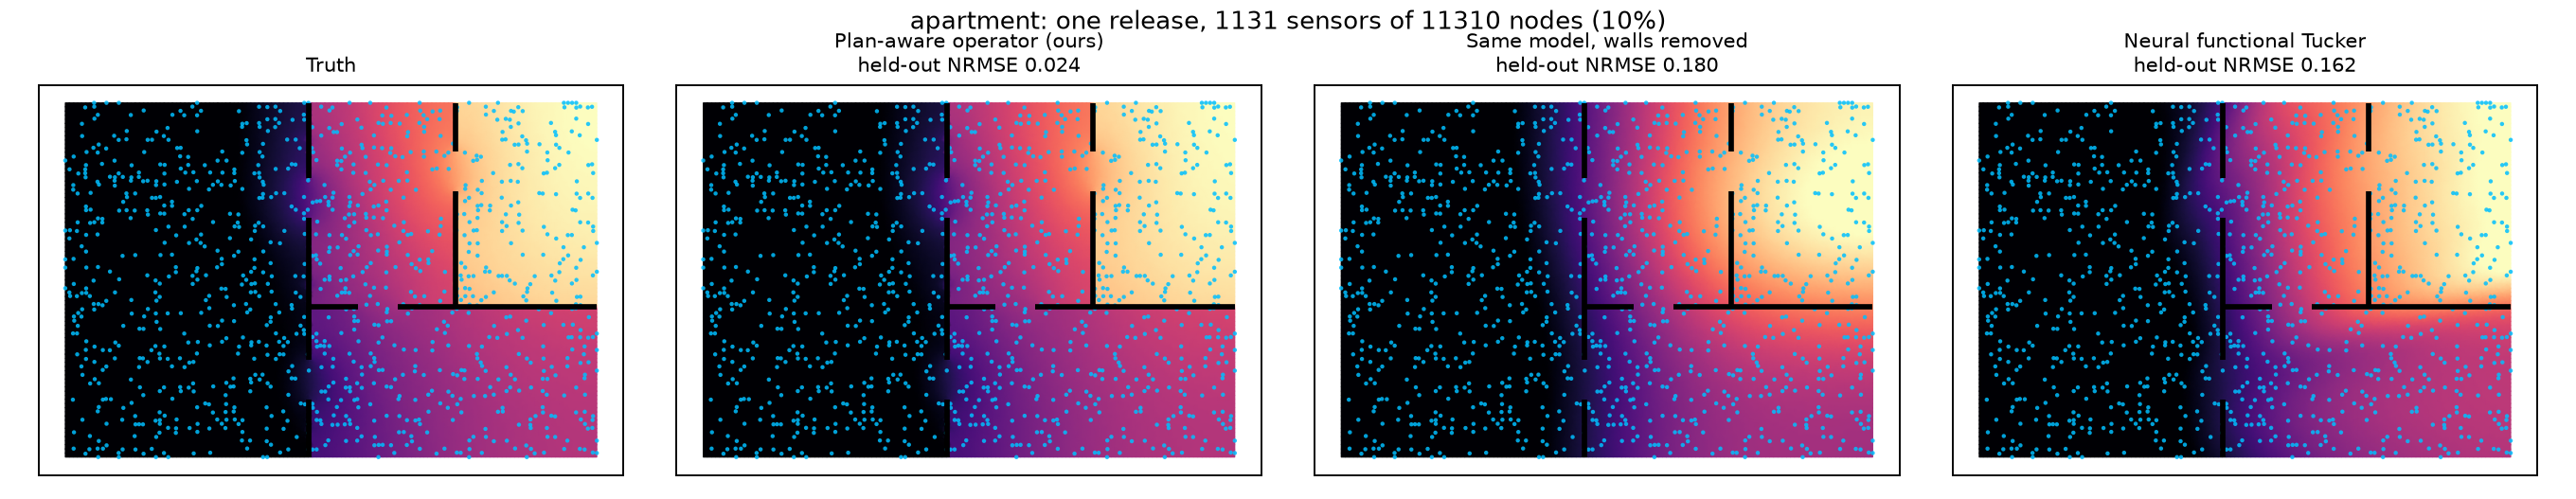
\includegraphics[width=\linewidth]{reconstruction_apartment.png}
\caption{同样 $1\,131$ 个传感器（$10\%$）下的重构。真值（左一）在墙处是一道\textbf{陡峭
的断层}；本文方法（左二）还原了它，而不知道墙的\emph{同一个模型}（左三）与坐标神经
网络（右一）都把浓度\textbf{抹过了墙}，在另一侧凭空造出不存在的污染。
绿点是传感器位置的采样（两侧拿到的完全相同）。}
\label{fig:recon}
\end{figure}

\subsection{几何信息是免费的，材料信息不是}

本文方法的可行性建立在一个不对称上：

\begin{center}
\begin{tabular}{@{}ll@{}}
\toprule
\textbf{通常已知（免费）} & \textbf{通常未知（需要测量）}\\
\midrule
楼层平面图、墙与门的位置 & 空气的有效扩散率\\
海岸线、岛屿轮廓 & 水体的实际粘性\\
设备布局与隔断图纸 & 局部湍流强度\\
\bottomrule
\end{tabular}
\end{center}

我们\textbf{只使用左列}。右列在生成真值时含有一个平滑的背景变化，而学习器对此
一无所知。这使得本方法的先验层级是\emph{几何先验}而非\emph{已知物理}——比
物理信息神经网络（PINN）一类方法的假设弱得多，也因此更容易在真实场景成立。

%===========================================================================
\section{任务设定}

\subsection{数据与观测}

给定张量 $\bY\in\Rb^{N_1\times N_2\times N_3}$ 与观测索引集 $\Om\subset
[N_1]\times[N_2]\times[N_3]$，$|\Om|/(N_1N_2N_3)$ 取 $2\%$ 到 $20\%$。
观测值带有噪声
\begin{equation}
y_{i}=\bY_{i}+\varepsilon_i,\qquad
\varepsilon_i\sim\mathcal N\!\big(0,\ (0.1\,\sigma_{\Om})^2\big),\qquad
i\in\Om,
\end{equation}
其中 $\sigma_\Om$ 是观测值的标准差。目标是重构\textbf{留出条目}上的值，
评价指标为
\begin{equation}
\mathrm{NRMSE}=\frac{\sqrt{\frac{1}{|\Om^c|}\sum_{i\in\Om^c}(\hat y_i-\bY_i)^2}}
{\mathrm{std}\big(\{\bY_i\}_{i\in\Om^c}\big)}.
\end{equation}
$\mathrm{NRMSE}=1$ 相当于用留出集均值作预测。

\subsection{学习器可见与不可见的信息}

\begin{itemize}
\item \textbf{可见}：网格（节点坐标与单元）、障碍物的位置与形状、边界条件类型、
观测索引集 $\Om$、以及 $\Om$ 上的带噪观测值。
\item \textbf{不可见}：背景材料参数的空间变化、留出条目的任何信息、真值使用的模态数。
\end{itemize}

这一条有单元测试守着：改变真值材料时，学习器的所有基必须\emph{逐位不变}。

\subsection{核心对照的设计}

本文所有主结果都建立在一个只差一件事的对照上：

\begin{center}
\begin{tabular}{@{}ll@{}}
\toprule
\code{geometry\_operator} & 算子知道障碍在哪里\\
\code{blind\_operator} & \textbf{同一个模型}，算子不知道障碍\\
\bottomrule
\end{tabular}
\end{center}

两者共享节点集、解码器、优化器、先验、闭式核后验、以及全部超参数。
唯一区别是装配算子时是否包含障碍。因此任何性能差异\textbf{只能}来自几何信息。

更重要的是\textbf{阴性对照}：在没有障碍的布局上，两个算子是\emph{同一个数学对象}，
优势必须精确为 $1.00$。这是整个论证的支点——它排除了"提出的模型本来就更好"这一
替代解释。

%===========================================================================
\section{方法}

\subsection{总体思路}

打个比方。要描述一栋楼里的温度分布，普通方法给模型一支笔，让它在整张平面图上随便画；
我们的做法是先根据平面图裁出一批"积木"——\textbf{每块积木都自动在墙处断开、在门洞处
连通}——然后让模型只能用这些积木拼。

拼出来的结果天然不穿墙，因为每块积木本身就不穿墙；而且要学的东西少一个数量级。

\begin{figure}[htbp]\centering
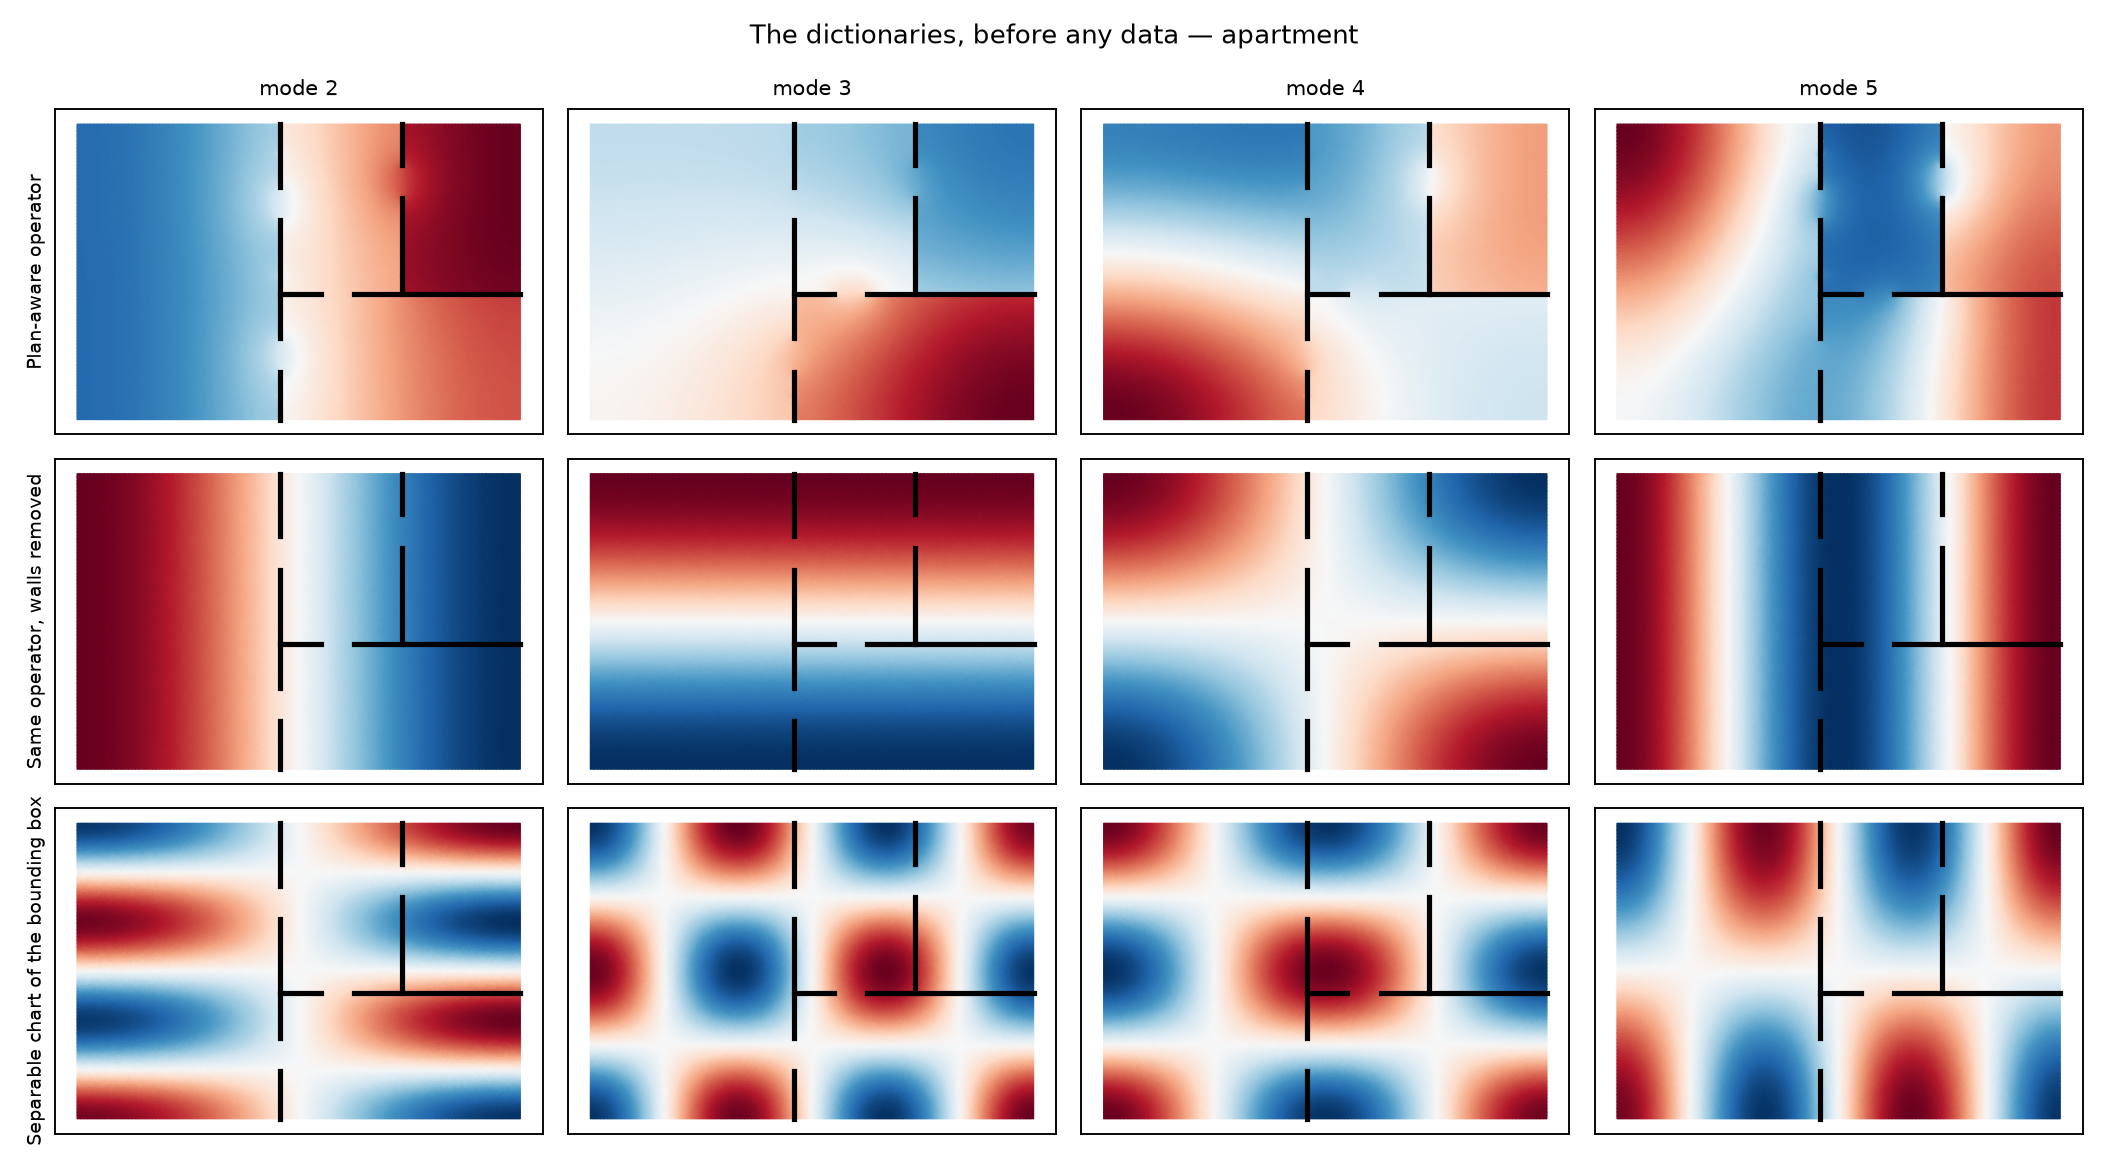
\includegraphics[width=\linewidth]{basis_apartment.png}
\caption{\textbf{拟合之前}的字典，不含任何数据。上行是本文的几何感知算子——特征函数
在墙处断开、在门洞处连通，房间成为自然的"块"；中行是\emph{忘了墙}的同一算子，给出
无视墙的平滑斜坡；下行是把楼当成矩形的可分基，完全盲目的棋盘格。
方法的全部内容就是"空间因子被允许长什么样"。}
\label{fig:basis}
\end{figure}

\subsection{算子及其谱基}

设域为 $\Om\subset\Rb^d$。取扩散型算子
\begin{equation}
\bA u=-\nabla\!\cdot\!\big(a(x)\nabla u\big)+\kappa u,
\end{equation}
$a(x)$ 为扩散系数，$\kappa$ 为反应率。障碍物实现为 $a(x)$ 取极小值的薄带
（对比度 $100{:}1$，理由见 \S\ref{sec:pitfalls}）。

\subsubsection{P1 有限元：那些"积木"是怎么算出来的}

把域剖成单纯形（二维三角形、三维四面体）。对每个节点 $i$ 定义\textbf{帽子函数}
$\varphi_i$：在节点 $i$ 上取 $1$，在其他所有节点上取 $0$，在每个单元内部线性变化。
这些函数张成所有分片线性连续函数的空间，于是任何这样的函数可写成
\begin{equation}
u(x)=\sum_i u_i\,\varphi_i(x),
\label{eq:nodal}
\end{equation}
其中 $u_i$ 是它在节点 $i$ 上的值。\textbf{函数与节点值向量一一对应}——这是后文
\S\ref{sec:continuous} 的基础。

在一个单元 $T$ 内用重心坐标 $\lambda_0,\dots,\lambda_k$ 描述。设顶点为
$p_0,\dots,p_k$，记边矩阵 $E=[p_1-p_0;\dots;p_k-p_0]\in\Rb^{k\times n}$。
由 $x-p_0=E^\top\lambda_{1:k}$ 两边左乘 $E$ 得
\begin{equation}
\lambda_{1:k}=(EE^\top)^{-1}E\,(x-p_0)
\quad\Longrightarrow\quad
\nabla\lambda_{1:k}=(EE^\top)^{-1}E,\qquad
\nabla\lambda_0=-\sum_{i\ge1}\nabla\lambda_i,
\end{equation}
梯度在单元内为常数。单元体积为 $|T|=\sqrt{\det(EE^\top)}/k!$，于是
\begin{equation}
K^T_{ij}=a_T\,|T|\,\nabla\lambda_i\!\cdot\!\nabla\lambda_j,
\qquad
M^T_{ij}=\frac{|T|}{(k+1)(k+2)}\big(1+\delta_{ij}\big),
\label{eq:element}
\end{equation}
累加到全局得稀疏矩阵 $K,M$。

\begin{principle}[同一公式覆盖三种几何]
$EE^\top$ 是\emph{诱导度量}。取 $k=n=2$ 是平面三角形，$k=n=3$ 是四面体，
而 $k=2,\,n=3$——三维空间中的曲面三角形——式~\eqref{eq:element} 自动给出
\textbf{Laplace–Beltrami 算子}。球面因此不需要任何特殊代码，只需要一张不同的网格。
\end{principle}

该性质有测试守着：球面的特征值必须是解析解 $l(l+1)=0,2,2,2,6,\dots$。

\subsubsection{谱基}

取广义特征问题的最低 $K$ 个解
\begin{equation}
K\phi_k=\lambda_k M\phi_k,\qquad
\lambda_1\le\cdots\le\lambda_K,\qquad
\Phi=[\phi_1,\dots,\phi_K]\in\Rb^{N\times K},
\end{equation}
并取\textbf{质量正交归一} $\Phi^\top M\Phi=I$。后者不是形式讲究：在非均匀网格上，
普通欧氏正交会让\emph{节点密度}而非\emph{函数频率}决定什么算低频。

实现使用移位反演 Lanczos，移位取 $\sigma=-10^{-6}$（纯 Neumann 算子在 $0$ 处奇异）。
代价与请求的模态数成正比而非 $N^3$：$642$ 节点的球面谱从稠密路径的 $32.0$ 秒降到
$0.11$ 秒，$40\,962$ 节点的球面稠密不可行、稀疏 $35.6$ 秒。两条路径在都能跑的网格上
给出\emph{逐位相同}的张量，特征值差 $5.7\times10^{-13}$。

\subsection{模型：分组算子先验 Tucker}

坐标划分成若干\textbf{组} $g$，每组配一个因子：
\begin{equation}
F_g=
\begin{cases}
\Phi_g W_g & \text{算子组：该组有可信算子}\\
T_g & \text{自由表：如"场景"这类枚举，没有算子可言}\\
\mathrm{MLP}_\theta(x_g) & \text{神经组：有坐标但无可信算子}
\end{cases}
\end{equation}
每组恰含一个张量轴时退化为逐轴模型。这一点很重要：方法\textbf{不要求}张量每一维
都有一条独立 PDE。

预测为
\begin{equation}
\hat y(i_1,i_2,i_3)=\sum_{r_1,r_2,r_3}\bG_{r_1r_2r_3}\prod_{m}\tilde F_m(i_m,r_m),
\end{equation}
其中 $\tilde F$ 是逐列单位 RMS 归一化后的因子。归一化让先验与尺度无关；代价是因子尺度
不可辨识，但它被核吸收，而核正是唯一有后验的对象。

\textbf{CP 是同一模型的对角核特例}：令 $R_1=R_2=R_3=R$、
$\bG_{r_1r_2r_3}=w_r\delta_{r_1r_2r_3}$ 即可。这样做的意义在于：CP 基线与本方法
共享优化器、归一化、先验和闭式后验，\textbf{两者的差异只能来自模型本身}。

\subsection{先验}

对算子组使用 Sobolev 谱罚
\begin{equation}
\mathcal R_g(W_g)=\frac{1}{K_gR_g}\sum_{k,r}(1+\lambda_{g,k})^{p}\,
\widetilde W_{g,kr}^{2},\qquad p=1.5,
\label{eq:sobolev}
\end{equation}
即高频模态付更高代价——$(1+\lambda_k)^p$ 正是 Sobolev 范数在特征基下的权重。

对自由表组（若给定罚算子 $P$）使用 $\operatorname{tr}(F^\top PF)$，其中 $P$ 满足
$\phi_k^\top P\phi_k=(1+\lambda_k)^p$。这构造出关键对照：\textbf{自由表付与谱因子
完全相同的频率代价，唯一差别是它不被限制在前 $K$ 个模态里}——这正是"是几何起作用
还是截断起作用"这个消融所需要的。

总目标为
\begin{equation}
\mathcal L=\frac{1}{|\Om|}\sum_{i\in\Om}\big(\hat y_i-y_i\big)^2
+\beta_{\mathrm{reg}}\Big[\overline{\bG^2}+\sum_g\mathcal R_g\Big],
\qquad \beta_{\mathrm{reg}}=2\times10^{-3}.
\label{eq:loss}
\end{equation}

\subsection{推断：两段式}

\paragraph{第一段（因子）} AdamW，学习率 $3\times10^{-3}$，权重衰减 $10^{-6}$，
梯度裁剪 $5.0$，$1500$ 步，冷随机初始化，无早停，但保留\emph{目标值最优}的检查点
而非最后一步的迭代。

\paragraph{第二段（核）} 固定因子后，模型对核是\textbf{线性}的。记
\begin{equation}
z(i)^\top=\Big(\tilde F_1(i_1,r_1)\tilde F_2(i_2,r_2)\tilde F_3(i_3,r_3)\Big)_{r_1r_2r_3}
\in\Rb^{p},\qquad p=R_1R_2R_3,
\end{equation}
即三个因子行的逐行 Kronecker 积（CP 情形为 Khatri--Rao 积，$p=R$）。取
$p(\bG)=\mathcal N(0,\alpha^{-1}I)$、$p(y\mid\bG)=\mathcal N(Z\mathrm{vec}(\bG),\beta^{-1}I)$，
标准结果给出
\begin{equation}
\Sigma=\big(\beta Z^\top Z+\alpha I\big)^{-1},
\qquad
\mu=\beta\,\Sigma\,Z^\top y .
\label{eq:posterior}
\end{equation}
$\alpha,\beta$ 用证据不动点（type-II 最大似然）估计。定义有效参数个数
$\gamma=p-\alpha\operatorname{tr}(\Sigma)$，迭代
\begin{equation}
\alpha\leftarrow\frac{\gamma}{\norm{\mu}^2},
\qquad
\beta\leftarrow\frac{|\Om|-\gamma}{\norm{y-Z\mu}^2}.
\label{eq:evidence}
\end{equation}

\begin{principle}[在特征基中迭代]
$Z^\top Z$ 在整个不动点循环中\emph{不变}，所以只做一次对角化
$Z^\top Z=V\Lambda V^\top$，此后每次迭代都在特征基下进行——协方差是对角的、
迹是求和、均值是逐元素缩放——把每次迭代从 $O(p^3)$ 降到 $O(p)$。
核为 $1920$ 时这是"整个拟合被这个循环主导"与"不被主导"的差别。
\end{principle}

预测方差为 $z^\top\Sigma z+\beta^{-1}$，再乘一个由留一残差得到的校准系数
（杠杆值修正，取 $95$ 分位除以 $1.96$，截断在 $[0.5,4]$）。因此误差棒是
\emph{经过校准}的，不是裸后验方差。

\paragraph{明确没有做的} 因子上没有后验。这是设计取舍，代价见 \S\ref{sec:pitfalls}
关于谱 ARD 的负结果。

\subsection{前向计算：不物化设计矩阵}

朴素实现显式构造 $Z$。当核有 $1920$ 个元素、观测有 $65$k 行时，$Z$ 是
$1.25\times10^8$ 个数（$500$ MB），且每个梯度步重建一次。正确做法是按模态依次收缩：
\begin{equation}
t^{(1)}_{n,r_2r_3}=\sum_{r_1}\tilde F_1\bG_{r_1r_2r_3},\quad
t^{(2)}_{n,r_3}=\sum_{r_2}\tilde F_2 t^{(1)}_{n,r_2r_3},\quad
\hat y_n=\sum_{r_3}\tilde F_3 t^{(2)}_{n,r_3}.
\end{equation}
结果完全相同（float32 下差 $2.4\times10^{-6}$，对角核精确为 $0$），算术量约 $2.4$ 倍少，
峰值内存降一个数量级。$1920$ 元素的核因此与 $96$ 元素的一样快。

\subsection{空间因子是一个函数，不是查找表}
\label{sec:continuous}

由式~\eqref{eq:nodal}，$\Phi$ 的每一列是一个 P1 函数，矩阵只是它的节点迹。
在任意点求值即重心插值：找到含 $x$ 的单元，
\begin{equation}
u(x)=\sum_{i\in T(x)}\lambda_i(x)\,u_i .
\end{equation}
因此本模型\textbf{与坐标神经网络一样可以在域内任意位置求值}，只是求值方式从"前向过
一个 MLP"换成"单元内重心插值"。

实测（$5\,520$ 节点上拟合，在 $4\,000$ 个\emph{非节点}位置查询，与独立的 $34\,355$
节点细网格真值比较）：非节点位置 NRMSE $=0.0278$，节点上 $=0.0265$，相差 $5\%$。

三个边界需要说清：(i) P1 插值在网格尺度上是二阶的，神经场原则上更光滑，但\emph{我们
在墙处的断裂是精确的}（它是从算子解出来的）；(ii) 域外无定义，而"墙外面没有场"本来
就是正确答案；(iii) 自由表不能插值——两个类别标签之间没有中点，代码对此报错而非静默
插值。

%===========================================================================
\section{算法}

\begin{algorithm}[htbp]
\caption{构造几何字典（离线，一次性，不接触数据）}
\label{alg:dict}
\begin{algorithmic}[1]
\Require 域 $\Om$；障碍集合 $\mathcal O$；基的列数 $K$
\Ensure 谱基 $\Phi\in\Rb^{N\times K}$（满足 $\Phi^\top M\Phi=I$）；特征值 $\lambda$
\State 剖分域：抖动格点 $+$ Delaunay \Comment{\code{irregular\_fem.build\_mesh}}
\State 学习器材料：$a(x)\!\leftarrow\!1$ 于背景，$a(x)\!\leftarrow\!10^{-2}$ 于 $\mathcal O$
       \Comment{\textbf{信息层级分界线}}
\State 装配 $K,M$：按式~\eqref{eq:element} 逐单元累加
       \Comment{\code{simplex\_fem.assemble\_sparse}}
\State 求最低 $K$ 个广义特征对：移位反演 Lanczos，$\sigma=-10^{-6}$
       \Comment{\code{sparse\_eigenpairs}}
\State \Return $\Phi,\lambda$
\end{algorithmic}
\end{algorithm}

\begin{algorithm}[htbp]
\caption{两段式拟合}
\label{alg:fit}
\begin{algorithmic}[1]
\Require 各组基 $\{\Phi_g,\lambda_g\}$；观测索引 $\Om$ 与观测值 $y$；
         秩 $(R_1,R_2,R_3)$；$p$；$\beta_{\mathrm{reg}}$；步数 $T$
\Ensure 因子参数 $\{W_g\}$；核后验 $(\mu,\Sigma)$；超参 $(\alpha,\beta)$；校准 $c$
\Statex \textbf{第 0 步：可观测性筛选（只读掩码，不读数据）}
\State $v_k\leftarrow\dfrac{\sum_{i\in\Sen}\phi_k(i)^2}{\sum_i\phi_k(i)^2}
        \Big/\dfrac{|\Sen|}{N}$；保留 $\{k:v_k\ge0.1\}\cup\{1\}$
\Statex \textbf{第一段：因子}
\For{$t=1,\dots,T$}
  \State $\tilde F_g\leftarrow\mathrm{normcol}(F_g)$ 对每组 $g$
  \State 按模态收缩求 $\hat y$（不物化 $Z$）
  \State 按式~\eqref{eq:loss} 求 $\mathcal L$，AdamW 更新，梯度裁剪 $5.0$
  \State 若 $\mathcal L$ 为历史最优则记录检查点
\EndFor
\State 载回最优检查点 \Comment{不是最后一步的迭代}
\Statex \textbf{第二段：核（闭式，无梯度）}
\State $Z^\top Z=V\Lambda V^\top$ \Comment{只分解一次}
\State $b\leftarrow V^\top Z^\top y$；$\alpha\leftarrow1$；$\beta\leftarrow25$
\For{$j=1,\dots,80$ 或至收敛}
  \State $\pi\leftarrow\beta\lambda+\alpha$；\;
         $\tilde\mu\leftarrow\beta\,b\oslash\pi$；\;
         $\gamma\leftarrow p-\alpha\sum_k\pi_k^{-1}$
  \State $\alpha\leftarrow\gamma/\norm{\tilde\mu}^2$；\;
         $\beta\leftarrow(|\Om|-\gamma)\big/
         \big(\norm{y}^2-2\tilde\mu^\top b+\sum_k\lambda_k\tilde\mu_k^2\big)$
\EndFor
\State $\Sigma\leftarrow V\mathrm{diag}(\pi^{-1})V^\top$；\;
       $\mu\leftarrow\beta V(b\oslash\pi)$
\State 由杠杆值修正的留一残差求校准系数 $c$
\State \Return $\{W_g\},\ \mu,\ \Sigma,\ \alpha,\ \beta,\ c$
\end{algorithmic}
\end{algorithm}

\begin{algorithm}[htbp]
\caption{预测（含任意位置）}
\label{alg:predict}
\begin{algorithmic}[1]
\Require 查询索引；因子 $\{\tilde F_g\}$；$(\mu,\Sigma,\beta,c)$；
         \textbf{可选}：查询坐标 $x$ 与网格
\Ensure 均值 $\hat y$ 与标准差 $\sigma$
\If{在网格节点上查询}
  \State $z(i)\leftarrow$ 因子行的逐行 Kronecker 积
\Else
  \State $\tilde F_3(x,\cdot)\leftarrow\sum_{i\in T(x)}\lambda_i(x)\tilde F_3(i,\cdot)$
         \Comment{重心插值，\S\ref{sec:continuous}}
  \State $z(x)\leftarrow$ 以插值行替换空间那一组后的 Kronecker 积
\EndIf
\State $\hat y\leftarrow z^\top\mu$；\quad
       $\sigma\leftarrow c\sqrt{z^\top\Sigma z+\beta^{-1}}$
\State \Return $\hat y,\ \sigma$
\end{algorithmic}
\end{algorithm}

\subsection{超参数及其来历}

\begin{table}[htbp]\centering\small
\caption{冻结的超参数值。每一个都有明确来历，而非试出来的。}
\begin{tabular}{@{}llll@{}}
\toprule
符号 & 配置键 & 值 & 怎么定的\\
\midrule
$K$ & \code{basis\_cutoff} & 逐家族 $16/32/48$ &
  \textbf{两条规则同时满足}（\S\ref{sec:diag}）\\
$(R_1,R_2,R_3)$ & \code{ranks} & $(12,10,16)$ &
  提到 headroom 落进 $1.0$–$1.5$ 为止\\
$p$ & \code{power} & $1.5$ & 沿用冻结的一维实验\\
$\beta_{\mathrm{reg}}$ & \code{reg} & $2\times10^{-3}$ & 同上\\
$T$ & \code{steps} & $1500$ & 收敛测试：$1500\to4000$ 无变化\\
障碍传导率 & \code{barrier} & $10^{-2}$ & 物理论证（\S\ref{sec:pitfalls}）\\
网格分辨率 & \code{resolution} & 逐家族 & 由最小几何特征尺度定\\
观测噪声 & \code{noise} & $0.10$ & 观测标准差的比例\\
\bottomrule
\end{tabular}
\end{table}

%===========================================================================
\section{拟合前诊断量}
\label{sec:diag}

这些量\textbf{在拟合之前}即可计算，只用真值张量、候选基和观测掩码。
它们是本方法区别于"试试看"的地方。

\paragraph{投影残差（基能否张成这个场）}
\begin{equation}
\varepsilon(\Phi)=\frac{\norm{\bY-\bY\times_3(QQ^\top)}_F}{\norm{\bY}_F},
\qquad Q=\mathrm{qr}(\Phi),
\end{equation}
即\textbf{偏差下限}。实现必须写成 $Q(Q^\top\bY)$ 而非 $(QQ^\top)\bY$，
否则要物化 $N\times N$ 的投影算子。

\paragraph{可观测性（这个模态在传感器上被激发吗）}
\begin{equation}
v_k=\frac{\sum_{i\in\Sen}\phi_k(i)^2}{\sum_i\phi_k(i)^2}\Big/\frac{|\Sen|}{N}.
\end{equation}
局域在薄障碍内部的模态，特征值是全谱\emph{最低}的，但传感器几乎不可能落在薄墙里。
这样的模态系数完全无约束，模型会用它外推出荒谬的值——我们实测到 NRMSE $1.246$、
预测范围 $[-74.8,\,77.8]$ 而真值在 $[-5.8,\,10.4]$，其可见度为
$v_5..v_8=0.004,\,0.001,\,0.001,\,0.002$。

\paragraph{Headroom（秩能否兑现这个基）}
\begin{equation}
\text{headroom}=\frac{\text{实际达到的 NRMSE}}{\text{该模型自身的投影残差}}.
\end{equation}
远大于 $1$ 意味着拟合是\emph{秩受限}的，此时任何关于函数空间的比较\textbf{不成立}
——所有方法被同一个与几何无关的天花板压着。健康值在 $1.0$–$1.5$。

\begin{principle}[两条 cutoff 规则必须同时满足]
\label{prin:cutoff}
(i) \textbf{近似能力对齐}：$K$ 要让几何感知的偏差下限跨设定可比（本文取 $\approx0.02$）；
(ii) \textbf{可辨识性}：$K\times R_3$ 不得超过传感器数 $|\Sen|$。
两条冲突时方法就在适用区之外。
\end{principle}

%===========================================================================
\section{实验}

\subsection{基准与协议}

\begin{table}[htbp]\centering\small
\caption{五个几何家族，共 19 种布局。每个家族含一个"无几何"的阴性对照。}
\begin{tabular}{@{}lllrr@{}}
\toprule
家族 & 几何机制 & 几何盲对照 & 节点数 & $K$\\
\midrule
\code{plane\_barrier} & 方形内的薄隔板 & 同一算子、去掉隔板 & $5\,520$ & 16\\
\code{plane\_domain} & 孔洞与凹角 & 无视孔洞的重新剖分 & $3\,941$–$5\,520$ & 16\\
\code{volume\_barrier} & 立方体内的隔墙 & 同一算子、去掉隔墙 & $8\,000$ & 48\\
\code{sphere} & 闭曲面曲率（浅水） & lat-lon 可分图表基 & $10\,242$ & 32\\
\code{floorplan} & 房间与门洞（米制） & 同一算子、去掉墙 & $11\,310$ & 16\\
\bottomrule
\end{tabular}
\end{table}

冻结配置：张量 $(12,12,N)$，观测 $10\%$，噪声 $10\%$，$\text{ranks}=(12,10,16)$，
$1500$ 步，五个全新种子 $201$–$205$。\textbf{没有选择/确认两段}，因为没有任何配置
是在这些数字上选的——障碍对比度、$K$、模态筛选、步数、分辨率全部由拟合前诊断或
收敛测试定下。

对照模型：\code{blind\_operator}（核心消融）、\code{flat\_chart}（按轴分解）、
\code{neural\_tucker} 与 \code{neural\_cp}（坐标网络）、
\code{cp\_als} 与 \code{tucker\_als}（TensorLy，SVD 初始化，秩用留出集开天眼挑选）、
\code{permuted}（打乱索引--算子对齐的破坏性对照）。

\subsection{主结果：核心消融}

\begin{table}[htbp]\centering\small
\caption{留出 NRMSE，$10\%$ 传感器观测，五个种子。
\textbf{前四行是阴性对照}：没有几何时两个算子是同一对象，优势必须为 $1.00$。}
\label{tab:main}
\begin{tabular}{@{}llrrrc r@{}}
\toprule
家族 & 布局 & ours & 去掉几何 & 倍数 & 配对胜 & 神经 Tucker\\
\midrule
\rowcolor{gray!12}
\code{plane\_barrier} & \code{open} & 0.021 & 0.021 & \textbf{1.00} & 2/5 & 1.50\\
\rowcolor{gray!12}
\code{plane\_domain} & \code{square} & 0.021 & 0.021 & \textbf{1.00} & 2/5 & 1.51\\
\rowcolor{gray!12}
\code{volume\_barrier} & \code{open} & 0.039 & 0.039 & \textbf{1.00} & 4/5 & 1.73\\
\rowcolor{gray!12}
\code{floorplan} & \code{open\_plan} & 0.018 & 0.018 & \textbf{1.00} & --- & 2.83\\
\midrule
\code{plane\_domain} & \code{center\_hole} & 0.020 & 0.035 & 1.73 & 5/5 & 1.56\\
\code{plane\_domain} & \code{two\_holes} & 0.020 & 0.048 & 2.40 & 5/5 & 2.16\\
\code{plane\_domain} & \code{L\_shape} & 0.019 & 0.046 & 2.39 & 5/5 & 1.79\\
\code{plane\_domain} & \code{U\_shape} & 0.019 & 0.045 & 2.35 & 5/5 & 1.83\\
\code{plane\_barrier} & \code{arc} & 0.055 & 0.167 & 3.07 & 5/5 & 2.72\\
\code{plane\_barrier} & \code{chamber} & 0.048 & 0.178 & 3.70 & 5/5 & 1.55\\
\code{plane\_barrier} & \code{labyrinth} & 0.051 & 0.227 & 4.47 & 5/5 & 1.95\\
\code{floorplan} & \code{corridor} & --- & --- & 4.51 & 5/5 & ---\\
\code{floorplan} & \code{apartment} & --- & --- & \textbf{8.23} & 5/5 & ---\\
\code{plane\_barrier} & \code{sealed\_4} & 0.029 & 0.267 & \textbf{9.19} & 5/5 & 2.54\\
\code{floorplan} & \code{lab\_suite} & --- & --- & \textbf{11.44} & 5/5 & ---\\
\code{sphere} & \code{open\_ocean} & 0.041 & 0.563 & \textbf{13.91} & 5/5 & 1.28\\
\midrule
\multicolumn{7}{@{}l@{}}{\footnotesize 已知例外：\code{volume\_barrier} 的三个带隔墙布局为
$0.99$–$1.48$，机制见 \S\ref{sec:limits}。}\\
\bottomrule
\end{tabular}
\end{table}

三点同时成立：

\begin{enumerate}
\item \textbf{四个阴性对照精确并列}，配对胜率是随机的（$2/5$、$4/5$）。这排除了
"提出的模型本来就更好"这一解释——差距只能来自几何。
\item \textbf{十五个带几何的布局在两种协议下全部 $5/5$ 获胜}，倍数 $1.73$–$13.91$。
\item \textbf{二维十个布局全部战胜坐标网络}（$1.50$–$2.72$ 倍），且参数少一个数量级
（$288$ 对 $2\,982$）。空间结构不需要学，几何已经给了。
\end{enumerate}

\subsection{经典方法在传感器采样下未定义}

\begin{table}[htbp]\centering\small
\caption{经典张量补全按协议分裂。SVD 初始化，秩用留出集开天眼挑选，跑满迭代。}
\begin{tabular}{@{}lcc@{}}
\toprule
& 随机缺失 $10\%$ & 传感器 $10\%$\\
\midrule
CP-ALS & $0.27$–$0.66$ & $\mathbf{1.000}$（所有布局、所有秩）\\
Tucker-HOOI & $0.27$–$0.66$ & $\mathbf{1.000}$（同上）\\
\bottomrule
\end{tabular}
\end{table}

未观测节点出现在零个方程中，故在那里精确输出零。同样两个例程在随机缺失下是正常对手
——两种采样问的是两个不同的问题。

\subsection{不是只对扩散有效}

同一套十个二维几何，把抛物型换成阻尼双曲型（$K=64$，随机缺失 $10\%$，三个种子）：

\begin{table}[htbp]\centering\small
\begin{tabular}{@{}lrrrr@{}}
\toprule
布局 & ours & 去掉几何 & 倍数 & 神经 Tucker\\
\midrule
\rowcolor{gray!12}
\code{open}（对照） & 0.096 & 0.096 & \textbf{1.00} & 1.31\\
\code{labyrinth} & 0.122 & 0.220 & 1.80 & 1.94\\
\code{arc} & 0.118 & 0.237 & 2.01 & 2.50\\
\code{sealed\_4} & 0.085 & 0.237 & \textbf{2.79} & 2.26\\
\bottomrule
\end{tabular}
\end{table}

\subsection{适用条件：几何必须仍然约束场}
\label{sec:condition}

给真值加入无散度胞流（速度在隔板内部为零，几何一如既往真实），学习器的算子、基、
网格、隔板全部不动：

\begin{table}[htbp]\centering\small
\begin{tabular}{@{}lrrrr@{}}
\toprule
布局 & Pe & ours & 去掉几何 & 倍数\\
\midrule
\multirow{2}{*}{\code{chamber}（有开口）} & 0 & 0.012 & 0.206 & \textbf{17.7}\\
 & 100 & 0.013 & 0.012 & \textbf{0.95}\\
\midrule
\multirow{2}{*}{\code{sealed\_4}（全密封）} & 0 & 0.026 & 0.279 & \textbf{10.7}\\
 & 100 & 0.033 & 0.215 & \textbf{6.5}\\
\bottomrule
\end{tabular}
\end{table}

\textbf{两条曲线终点不同才是结论。} 对流本身并不破坏算子先验：全密封布局在对流强过
扩散一百倍时仍有 $6.5$ 倍优势，因为再快的输运也过不去一堵封死的墙；有开口的布局则被
对流把场直接搬过开口，优势精确归零。

\begin{principle}[适用条件]
\textbf{几何必须仍然约束场能去哪里。动力学能绕开的障碍，不再是几何。}
\end{principle}

两个外部真实数据集落在条件之外，结果与条件一致：RealPDEBench 圆柱绕流（PIV 实测，
$\mathrm{Re}\,1\,875$–$11\,625$）为 $1.00$–$1.08$ 倍；CFDBench 方腔流 24 种长宽比
为 $0.74$–$1.07$ 倍。圆柱是开放通道里的孤立小障碍，方腔是开放盒子——流体想去哪去哪，
没有约束可供算子编码。\textbf{这不是方法失败，是问题不在适用区，而且该判断在跑任何
模型之前就能做出。}

\subsection{应用：几何值多少个传感器}

\begin{table}[htbp]\centering\small
\caption{\code{floorplan/apartment}（$11\,310$ 节点，三个种子）。}
\begin{tabular}{@{}rrrr@{}}
\toprule
传感器 & ours & 去掉几何 & 神经 Tucker\\
\midrule
$113$（$1\%$） & \textbf{0.040} & 0.194 & 0.228\\
$566$（$5\%$） & 0.025 & 0.180 & 0.172\\
$2\,262$（$20\%$） & 0.020 & 0.177 & 0.160\\
\bottomrule
\end{tabular}
\end{table}

\begin{figure}[htbp]\centering
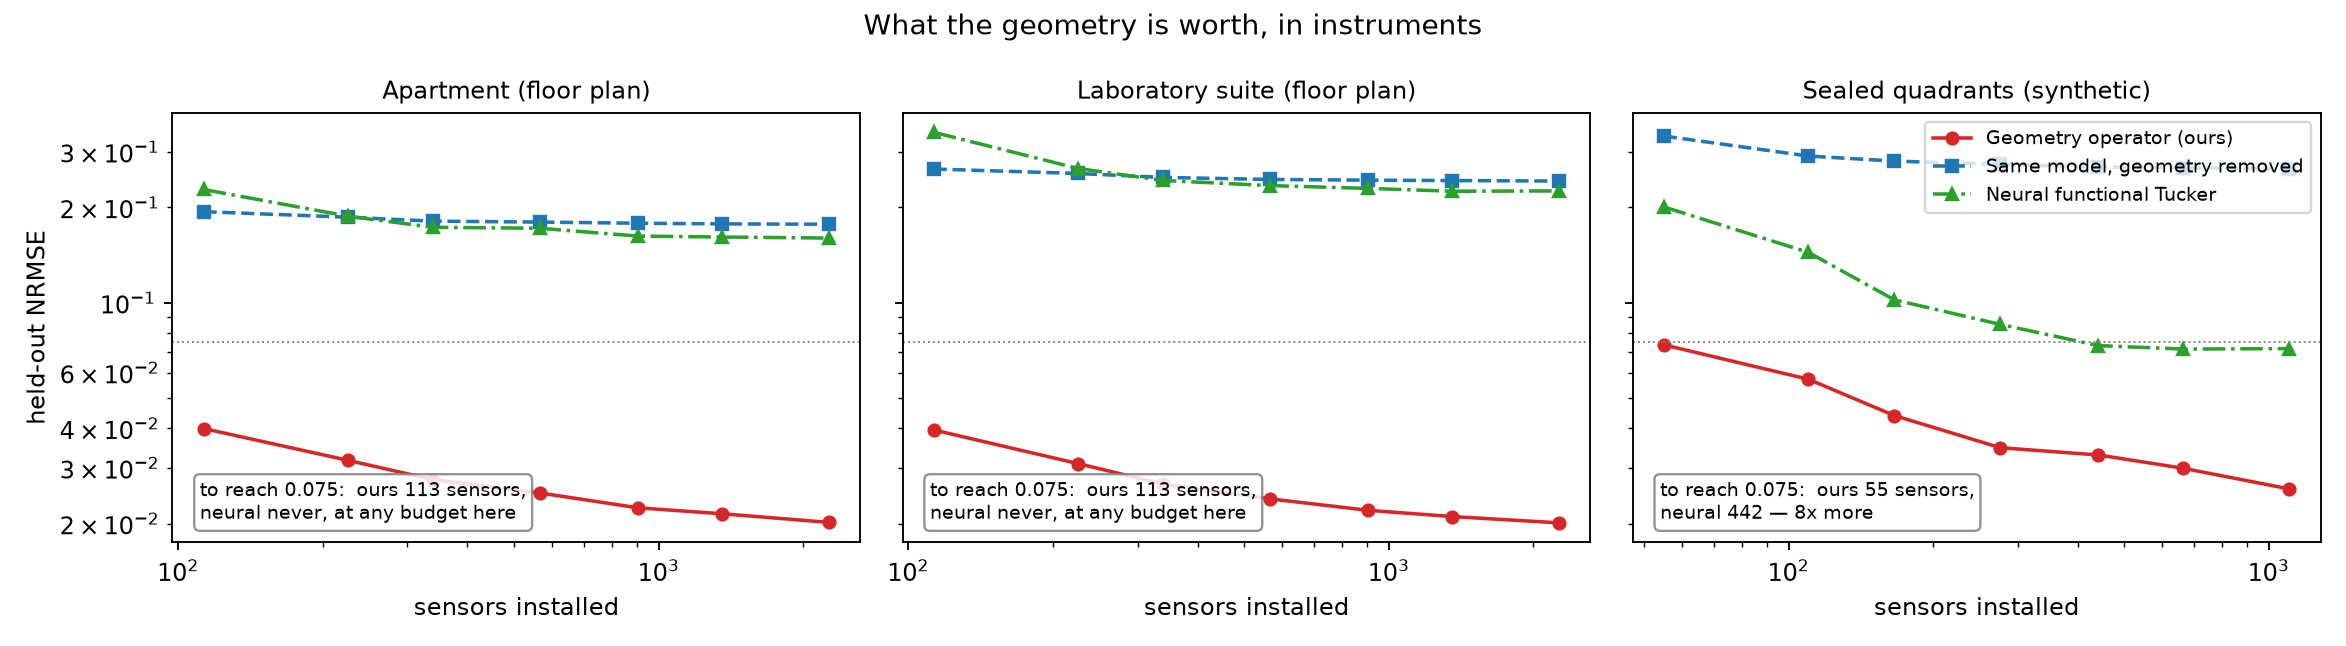
\includegraphics[width=\linewidth]{sensor_budget.png}
\caption{精度对传感器数量。\textbf{红线持续下降，蓝绿两条早早躺平。}
两个楼层平面上基线在任何测试预算下都达不到目标精度；合成布局上它们最终能到，
代价是 $8$ 倍传感器。}
\label{fig:budget}
\end{figure}

\textbf{基线在 $20$ 倍预算下仍达不到我们 $1\%$ 预算的精度}，而且从 $1\%$ 到 $20\%$
几乎不动（$0.194\to0.177$）。它们不是数据不够，是函数空间放不下墙上的断层，加传感器
补不上。合成的 \code{sealed\_4} 上基线最终能追上，代价是 $8$ 倍传感器。

%===========================================================================
\section{已知边界与踩过的坑}
\label{sec:pitfalls}
\label{sec:limits}

\paragraph{三维强隔板布局}
坐标网络更好（$0.51$–$0.85$ 倍）。机制清楚：三维达到同等近似质量的模态数按 $k^d$ 增长，
而 $K$ 被可辨识性顶死（$8\,000$ 节点、$800$ 传感器、$48\times16=768$ 已贴边）。
消融在最好配置上\emph{也最强}（$1.50$ 倍），说明卡住的是截断而非几何。

\paragraph{秩从别的实验照搬（代价最大的一个）}
$\text{ranks}=(4,4,6)$ 来自 $18\times24\times24$ 的一维实验，被原样搬到 $5\,000$–$11\,000$
节点的网格上从未复查。后果是整张主表被低估：\code{sealed\_4} 的消融从 $2.98$ 变成
$9.73$ 倍，对神经方法从 $1.26$ 变成 $2.68$ 倍。Headroom 就是为了防止此类问题复发。

\paragraph{分辨率未按障碍尺度校验（犯了两次）}
障碍比一个单元还薄时结果不可信，\emph{且偏差方向不可预测}：一次让隔板显得更厚而
\textbf{夸大}优势（$6.28\to$ 收敛值 $3.2$–$4.0$），一次让墙漏水而\textbf{低估}优势
（分辨率 $90$ 给 $3.4/4.0/10.1$，$130$ 给 $5.2/9.9/13.9$）。

\paragraph{障碍对比度}
$10^{-3}$ 时隔板自身的弛豫比场还慢，它变成独立的慢子系统，任何截断基都得把前几个模态
花在墙里面。$10^{-2}$（$100{:}1$）才是方法适用的区间。

\paragraph{谱 ARD 无法剪枝（结构性）}
点估计的 ARD 不动点缺少后验协方差项，罚项对每列恒为常数，什么都剪不掉。要真正剪枝
需要因子上的后验，而那正是本方法明确不做的部分。

\paragraph{基线初始化}
Tucker-HOOI 在随机初始化下发散到 NRMSE $3$–$20$。看上去像大幅领先，实际是基线坏了。
换 SVD 初始化后它是正常对手。\textbf{基线必须以最好状态出场。}

%===========================================================================
\section{相关工作定位}

\paragraph{张量分解与补全} 我们不提出新的分解结构，而是\textbf{约束因子所在的函数空间}。
在随机缺失下经典方法是正常对手；在传感器采样下它们的问题是未定义的——这是\emph{结构性}
对比，而非精度差距。

\paragraph{连续/函数型张量分解与隐式神经表示} 同样让因子是空间的函数，但\textbf{函数
空间的来源不同}：它们从数据里学出空间结构，我们直接从已知几何解出来。参数量差一个
数量级，且坐标网络对"哪些点在物理上相邻"没有先验——这正是它把浓度抹过墙的原因。

\paragraph{图 Laplacian 正则与流形学习} 这是最近的邻居，必须正面处理。区别有二：
(i) 我们的算子来自\emph{已知的物理几何}（有限元装配、真实边界条件与材料对比度），
不是从数据估计的相似度图；(ii) 我们做了 $2\times2$ 消融把"几何"与"表示形式"分开，
结论是\textbf{几何是活性成分}，而\textbf{截断是让几何可用的那一步}。

\paragraph{物理信息机器学习与算子学习} 信息层级不同：我们\textbf{不假设已知方程}，
只假设\textbf{已知几何}。这比 PINN 一类的假设弱得多，也因此更容易在真实场景成立。

%===========================================================================
\section{可复现性}

全部主表数据由代码生成，\textbf{不依赖任何外部文件}，装好
\code{torch/numpy/scipy/tensorly} 即可在任何机器上复现，不需要网格库。

\begin{verbatim}
export PYTHONPATH=src
python -m pytest -q                    # 64 项
python experiments/check_install.py    # 秒级；无障碍时比值必须精确为 1.00
python experiments/run_geometry_main.py --config configs/main.yaml \
       --families plane_barrier --output results/my_run
\end{verbatim}

超参数全部位于 \code{configs/*.yaml}；命令行覆盖文件，合并结果写入产物的
\code{configuration} 字段，因此一个数字永远不会被归因到它没有真正使用过的设定上。

详细文档见 \code{docs/HANDOVER\_ZH.md}（方法、推导、算法表、从零跑动指南、
全部实验设定）与 \code{docs/DATASETS.md}（数据来源与从零重建）。

\end{document}
